\item Buzz data source Module:

This module is responsible for sourcing data from the external cs database (Read Access) and using it for authentication and representation purposes.


\textbf{Use Cases}
\begin {itemize}


\item {Login and Administrative user}\\
This is the service that will authenticate against the cs data source where authentication credentials are stored

\begin {itemize}
\item Pre-conditions:\\
-should connect to CS data source (LDAP) (Not implemented-The system does not connect or acquire data from the computer science database )\\
        -user exists in ldap with provided authentication details (Implemented-The system has users that can connect to the system but are not in the cs data source, dummy users were created to provide the login functionality)\\
\item Post-conditions:\\
userID returned (not implemented-Code was found but no functionality)  
\end {itemize}

 
\begin{figure}[h!]
  \centering
    \reflectbox{%
      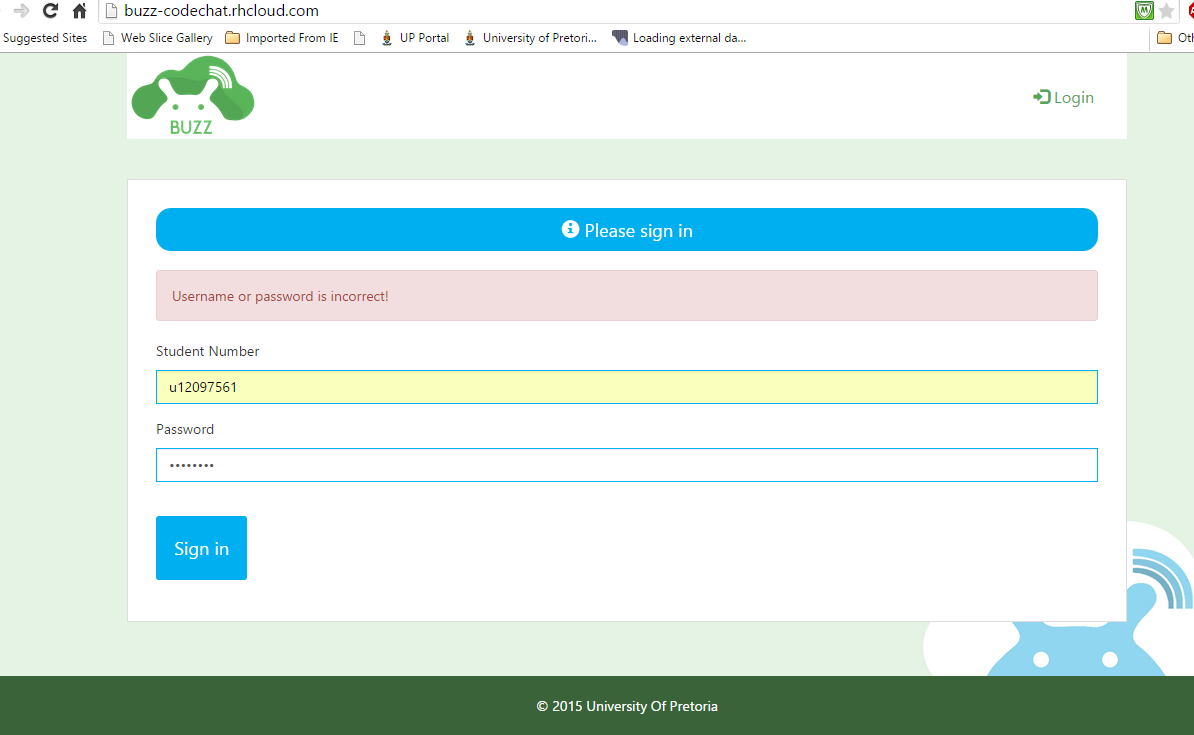
\includegraphics[width=0.5\textwidth]{loginadministrativeerror}}
  \caption{result to a user from the cs database trying to login }
\end{figure}


\begin{figure}[h!]
  \centering
    \reflectbox{%
      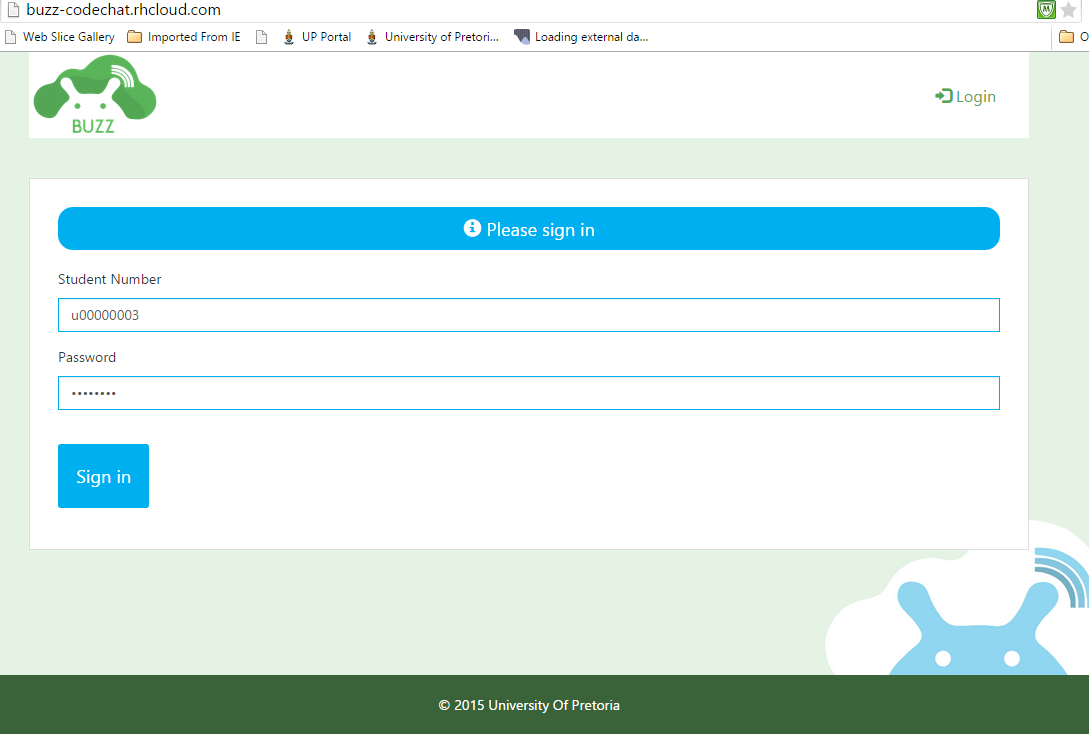
\includegraphics[width=0.5\textwidth]{loginadministrative(whatBdid)}}
  \caption{result to a dummy user not in the cs database trying to login }
\end{figure}

 
\item {getUsersRolesForModule}\\
This service is to query the user roles for a particular user\\


\begin {itemize}
\item Pre-conditions:\\
-should connect to CS data source (LDAP) (not implemented-No modules from cs data source where found , only one hard coded one)\\
        -user exists in ldap with provided authentication details (Not Implemented)\\
\item Post-conditions:\\
userID returned (not implemented)  
\end {itemize}


\begin{figure}[h!]
  \centering
    \reflectbox{%
      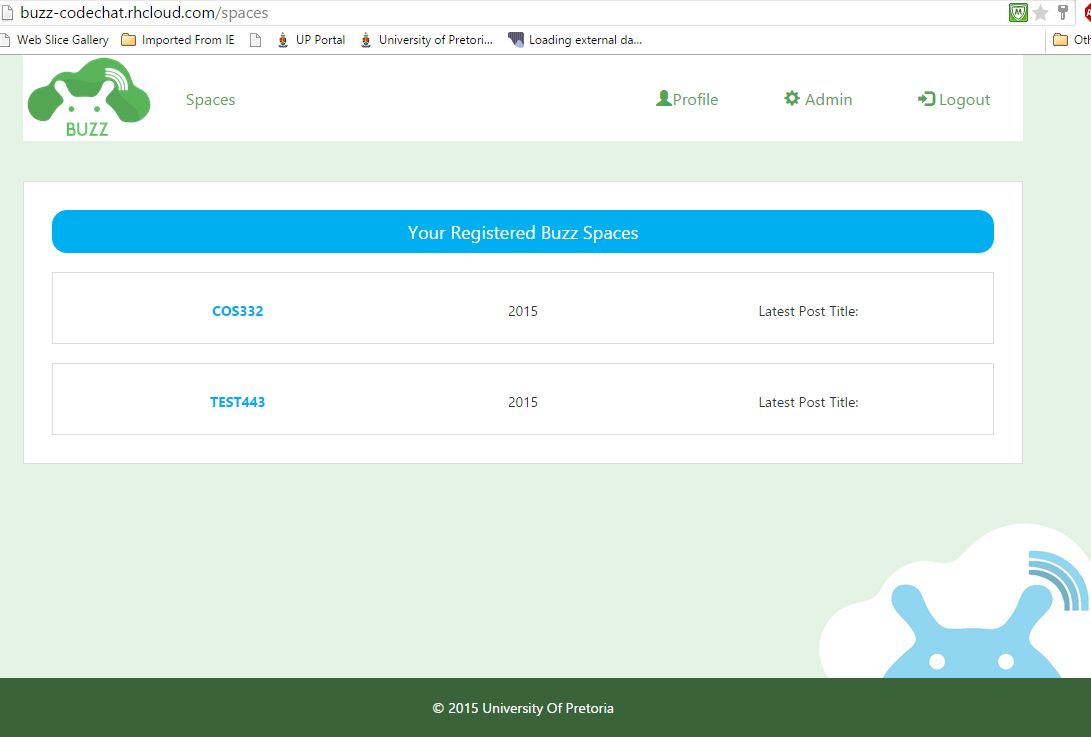
\includegraphics[width=0.5\textwidth]{modulesprovided}}
  \caption{result to a dummy user not in the cs database trying to login }
\end{figure}

 
\begin {itemize}
\item {GetUsersWithRole}\\
This service is required to retrieve al the users which have a role for a particular module
\\

\item Pre-conditions:\\
-should connect to CS data source (LDAP) (not implemented) No code found and no administrative users on site\\
 \begin{figure}[h!]
  \centering
    \reflectbox{%
      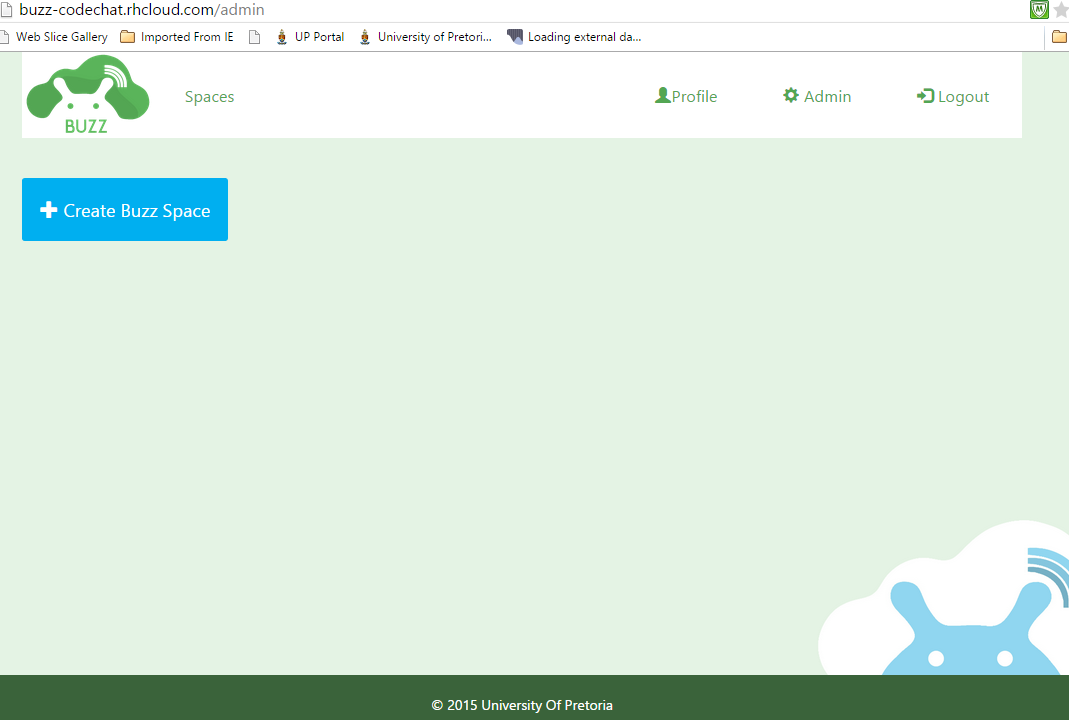
\includegraphics[width=0.5\textwidth]{userswithroles}}
  \caption{result to a dummy user not in the cs database trying to login }
\end{figure}   


 \end {itemize}  
\end {itemize}